\scanpage{133}

c) Let $X$ be a \deleted{complete}\inserted{proper} scheme over a field $k$, suppose $H^{\unsure{0|o}}(X,\underline{O}_{X})=k$. The category $\inserted{C}$ of coherent sheaves on $X$ is a category with $\unsure{\otimes|\Omega},\handwritten{\unsure{\phi|\varphi}},\handwritten{\unsure{\psi|\varphi|\mu}},$ \deleted{Hom} $1$, internal \uline{Hom}, 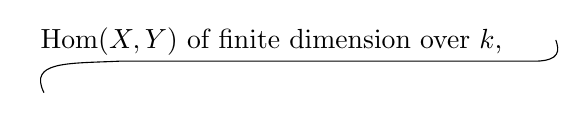
\begin{tikzpicture}[baseline=-.6ex,x=1cm,y=1cm]
\node[anchor=west,inner sep=0] at (0,.4) {\inserted{\handwritten{$\mathrm{Hom}(X,Y)$ of finite dimension over $k$,}}};
\draw (.05,-.25) .. controls (-.15,.15) and (.35,.12) .. (1,.15) -- (6.3,.15) .. controls (6.6,.16) and (6.6,.28) .. (6.55,.42);
\end{tikzpicture} but the homomorphism $\overset{\handwritten{\unsure{\vee|\nu|v}}}{X}\otimes Y\handwritten{\simeq}\underline{\mathrm{Hom}}(X,Y)$ \uline{is not an isomorphism}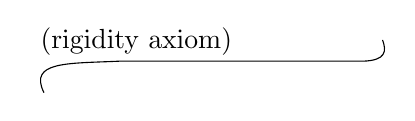
\begin{tikzpicture}[baseline=-.6ex,x=1cm,y=1cm]
\node[anchor=west,inner sep=0] at (0,.4) {\inserted{(rigidity axiom)}};
\draw (.05,-.25) .. controls (-.15,.15) and (.35,.12) .. (1,.15) -- (4.1,.15) .. controls (4.4,.16) and (4.4,.28) .. (4.35,.42);
\end{tikzpicture}. This is why there is no reason to expect a true Galois theory of $\rlap{\(X\)}C$. There are fiber functors associated with the various points of $X$ (not necessarily closed), to $x$ corresponds a fiber functor defined over $k(x)$; probably\deleted{i} there are no others up to isomorphism (to be checked). They\deleted{s} have all the compatibilities, but \uline{they are not exact}, \deleted{To remedy this} \uline{nor faithful}. To remedy the failure of exactness, without $C$ ceasing to be abelian (otherwise one would take locally free Modules only !), one can fix an open subset $U\quad X$ and define $C$ by taking coherent \unsure{\rlap{s}S|S}heaves which, on $U$, are equipped with a stratification relative\rlap{e}ly to $k$: every point $x\handwritten{\in}\rlap{\(M\)}U$ provides an exact fiber functor. However, if $U\handwritten{\not}=X$, this functor will not be faithful. Of course, if $U=X$, the rigidity axiom is satisfied, and one knows that one has a Galois theory. It must follow from the latter that $C$ has no fiber functor (compatible with all the data) over an extension of $k$ (for otherwise the rigidity axiom would be \rlap{s}\kern.35em atisfied).

\uline{To be proved:} Let $C$ be an 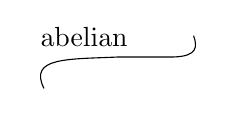
\begin{tikzpicture}[baseline=-.6ex,x=1cm,y=1cm]
\node[anchor=west,inner sep=0] at (0,.4) {\inserted{abelian}};
\draw (.05,-.25) .. controls (-.15,.15) and (.35,.12) .. (1,.15) -- (1.7,.15) .. controls (2.0,.16) and (2.0,.28) .. (1.95,.42);
\end{tikzpicture} category with biadditive $\otimes_{\deleted{\unsure{k|x}}}$, $\handwritten{\phi},\handwritten{\psi},1,{}^{\handwritten{\vee}}$ and rigidity. Then a) $\inserted{k=}\mathrm{End}(\unsure{\rlap{\(4\)}1|\mathbb{1}|1})$ is an absolutely flat ring, hence a finite product of \deleted{orops} fields if it is noetherian. b) The $\mathrm{Hom}(\rlap{\(C\)}X,Y)$ are finitely presented modules 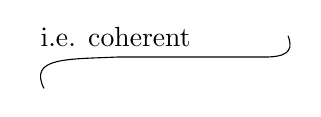
\begin{tikzpicture}[baseline=-.6ex,x=1cm,y=1cm]
\node[anchor=west,inner sep=0] at (0,.4) {\inserted{i.e. coherent}};
\draw (.05,-.25) .. controls (-.15,.15) and (.35,.12) .. (1,.15) -- (2.9,.15) .. controls (3.2,.16) and (3.2,.28) .. (3.15,.42);
\end{tikzpicture} \rlap{(}over $k$ (NB finitely presented modules over $k$ form an abelian category, in fact $k$ is a ``coherent'' ring\unsure{\rlap{,})|)}. c) \deleted{Every subcategory of $C$ stable under everything and with \unsure{engend}} $C$ is an inductive limit of subcategories (in gen\handwritten{\unsure{e|\rlap{u}e}}ral not full) stable under everything, including kernels, cokernels, ${}^{\handwritten{\vee}}$, $\otimes$, and corresponding to rings $k_{i}$ which are \deleted{sums} products of fields. d) The case of a product of fields reduces to that of a field.
% archive sheet number: 132
